\documentclass[../mathNotesPreamble]{subfiles}

\providecommand{\relscalefact}{1.4}
\begin{document}
\relscale{\relscalefact}
  \section{6.1: Graphs of the Sine and Cosine Functions}

  \begin{center}
    \begin{tikzpicture}[
      declare function={
        f(\x)=cos(deg(\x*pi));
        g(\x)=sin(deg(\x*pi));
        a=1/6; b=1/4; c=1/3;
        },
        nodeLabel/.style={pos=0.5, inner sep=5pt},
        every pin/.style={text=black, fill=white, opacity=0.85, text opacity=1},
        every pin edge/.style={black!50, line width=0.5pt},
      ]
      \begin{groupplot}[
        group style={group size=1 by 2, vertical sep=20mm},
        axis lines=center,
        axis line style={->},
        xmin=0, xmax=2,
        ymin=-1, ymax=1,
        xtick={-2, -1.5, ..., 2},
        xticklabels={$-2\pi$, $-\dfrac{3\pi}{2}$,$-\pi$, $-\dfrac{\pi}{2}$, ,
            $\dfrac{\pi}{2}$,$\pi$, $\dfrac{3\pi}{2}$, $2\pi$},
        minor x tick num=1,
        ytick={-1,1},
        ylabel=,
        enlargelimits={abs=0.05},
        height=\axisdefaultheight, width=0.95\linewidth,
        ticklabel style={font=\normalsize,inner sep=5pt,fill=white,opacity=1.0, text opacity=1},
        every axis plot/.append style={domain=0:2},
        clip=false,
        ]
        \nextgroupplot[xlabel=$\sin(x)$, xlabel style={at={(ticklabel* cs:1)},anchor=north west}]
          \addplot[<->] {g(x)};
          \addplot[soldot] coordinates{(a,{g(a)})}
            node[nodeLabel, pin=180:$\parens{\frac{\pi}{6},\frac{1\vphantom{\sqrt{3}}}{2}}$] {};
          \addplot[soldot] coordinates{(b,{g(b)})}
            node[nodeLabel, pin=135:$\parens{\frac{\pi}{4},\frac{\sqrt{2}}{2}}$] {};
          \addplot[soldot] coordinates{(c,{g(c)})}
            node[nodeLabel, pin=90:$\parens{\frac{\pi}{3},\frac{\sqrt{3}}{2}}$] {};
        \nextgroupplot[xlabel=$\cos(x)$, xlabel style={at={(ticklabel* cs:1)},anchor=north west}]
          \addplot[<->] {f(x)};
          \addplot[soldot] coordinates{(a,{f(a)})}
            node[nodeLabel, pin=90:$\parens{\frac{\pi}{6},\frac{\sqrt{3}}{2}}$] {};
          \addplot[soldot] coordinates{(b,{f(b)})}
            node[nodeLabel, pin=45:$\parens{\frac{\pi}{4},\frac{\sqrt{2}}{2}}$] {};
          \addplot[soldot] coordinates{(c,{f(c)})}
            node[nodeLabel, pin=0:$\parens{\frac{\pi}{3},\frac{1\vphantom{\sqrt{3}}}{2}}$] {};
      \end{groupplot}
    \end{tikzpicture}
  \end{center}

  \vspace*{2\baselineskip}
  \hspace*{\stretch{1}}
  \textcolor{blue}{\href{https://www.desmos.com/calculator/iwynbgwx8e}{\underline{Animated graphs}}}
  \pagebreak

  \noindent%
  Recall that 
  \begin{itemize}
    \item $\sin(\theta)$ and $\cos(\theta)$ have period $2\pi$,
    \item $\sin(\theta)$ is an odd function, and
    \item $\cos(\theta)$ is an even function:
  \end{itemize}
  \vspace*{\stretch{1}}
  
  \begin{center}
    \begin{tikzpicture}[
      declare function={
        f(\x)=cos(deg(\x*pi));
        g(\x)=sin(deg(\x*pi));
        a=pi/6; b=pi/4; c=pi/3;
        },
        nodeLabel/.style={pos=0.5, inner sep=5pt},
        every pin/.style={text=black, fill=white, opacity=0.85, text opacity=1},
        every pin edge/.style={black!50, line width=0.5pt},
      ]
      \begin{groupplot}[
        group style={group size=1 by 2, vertical sep=20mm},
        axis lines=center,
        axis line style={->},
        xmin=-2, xmax=3,
        ymin=-1, ymax=1,
        xtick={-2,-1,...,3},
        xticklabels={$-2\pi$, $-\pi$,  , $\pi$, $2\pi$, $3\pi$},
        minor x tick num=1,
        ytick={-1,1},
        ylabel=,
        enlargelimits={abs=0.15},
        height=\axisdefaultheight, width=0.95\linewidth,
        ticklabel style={font=\normalsize,inner sep=5pt,fill=white,opacity=1.0, text opacity=1},
        every axis plot/.append style={domain=-2:3},
        clip=false,
        ]
        \nextgroupplot[xlabel=$\sin(x)$, xlabel style={at={(ticklabel* cs:1)},anchor=north west}]
          \addplot[<->] {g(x)};
          \draw[dashed, red, line width=1pt] (0,-1) rectangle (2,1);
        \nextgroupplot[xlabel=$\cos(x)$, xlabel style={at={(ticklabel* cs:1)},anchor=north west}]
          \addplot[<->] {f(x)};
          \draw[dashed, red, line width=1pt] (0,-1) rectangle (2,1);
      \end{groupplot}
    \end{tikzpicture}
  \end{center}
  \vspace*{\stretch{1}}
  \pagebreak

  \noindent%
  Recall from \hyperref[sec:transFuncs]{transformations of functions}:
%  \cref{sec:transFuncs}
    \[af(bx-h)+k\]
  We have that $f(x)$ is
  \begin{tasks}[style=itemize](2)
    \task stretched vertically by $a$
    \task shifted right by $h$
    \task stretched horizontally by $\sfrac{1}{b}$
    \task shifted vertically by $k$
  \end{tasks}
  \vspace*{\stretch{1}}

  \begin{center}
    \begin{tikzpicture}[
      declare function={
        g(\x)=sin(deg(\x*pi));
        A=0.5; B=1.5; C=2/3; D=-0.5;
        },
        nodeLabel/.style={pos=0.5, inner sep=5pt},
        every pin/.style={text=black, fill=white, opacity=0.85, text opacity=1},
        every pin edge/.style={black!50, line width=0.5pt},
      ]
      \begin{groupplot}[
        group style={group size=2 by 2,horizontal sep=25mm,vertical sep=22.5mm},
        axis lines=center,
        axis line style={->},
        xmin=-2, xmax=2,
        ymin=-1, ymax=1,
        xtick={-2,-1,...,2},
        xticklabels={$-2\pi$, $-\pi$,  , $\pi$, $2\pi$},
        minor x tick num=1,
        ytick={-1,1},
        ylabel=,
        enlargelimits={abs=0.15},
        height=\axisdefaultheight, width=0.45\linewidth,
        ticklabel style={font=\normalsize,inner sep=5pt,fill=white,opacity=1.0, text opacity=1},
        every axis plot/.append style={domain=-2:2},
        ]
        \nextgroupplot[title=$\sin(x)$ vs. $\frac{1}{2}\sin(x)$]
          \addplot[<->] {g(x)};
          \addplot[<->, red] {A*g(x)};
          \pgfplotsinvokeforeach{-1.5, -0.5, 0.5, 1.5}{
            \draw[black!50, shorten <=5pt, shorten >=5pt, ->] 
              (axis cs: #1, {g(#1)}) -- (axis cs: #1, {A*g(#1)});
          }
        \nextgroupplot[title=$\sin(x)$ vs. $\sin\parens{x-\dfrac{2\pi}{3}}$]
          \addplot[<->] {g(x)};
          \addplot[<->, red] expression[domain=-2+C:2+C] {g(x-C)};
          \pgfplotsinvokeforeach{-1.7, -0.7, 0.3, 1.3}{
            \draw[black!50, shorten <=5pt, shorten >=5pt, ->] 
              (axis cs: #1, {g(#1)}) -- (axis cs: #1+C, {g(#1)});
          }
        \nextgroupplot[title=$\sin(x)$ vs. $\sin\parens{\dfrac{3x}{2}}$]
          \addplot[<->] {g(x)};
          \addplot[<->, red] expression[domain=-2/B:2/B] {g(B*x)};
          \pgfplotsinvokeforeach{-1.9, -1.3, -0.75, 0.75, 1.3, 1.9}{
            \draw[black!50, shorten <=1pt, shorten >=1pt, ->] 
              (axis cs: #1, {g(#1)}) -- (axis cs: #1/B, {g(#1)});
          }
        \nextgroupplot[title=$\sin(x)$ vs. $\sin(x)-\frac{1}{2}$]
          \addplot[<->] {g(x)};
          \addplot[<->, red] {g(x)+D};
          \pgfplotsinvokeforeach{-1.75, -0.75, 0.25, 1.25}{
            \draw[black!50, shorten <=5pt, shorten >=5pt, ->] 
              (axis cs: #1, {g(#1)}) -- (axis cs: #1, {g(#1)+D});
          }
      \end{groupplot}
    \end{tikzpicture}
  \end{center}
  \pagebreak

  \begin{defn*}[Sinusoidal functions]
    A \textbf{sinusoidal function} is a function that has the same general shape as a sine or cosine function. The general forms of sinusoidal functions are
      \[y=A\sin\parens{Bx-C}+D \quad \textnormal{ and } \quad y=A\cos\parens{Bx-C}+D,\]
    where
    \begin{itemize}
      \item $A$ determines the amplitude,
      \item $B$ determines the period,
      \item $C$ determines the phase shift, and
      \item $D$ determines the vertical shift.
    \end{itemize}
  \end{defn*}
  \begin{ex*}
    Identify the amplitude, period, phase shift, and vertical shift of
      \[3\sin\parens{2x}+1\]
    and sketch the graph:
    \vspace*{\stretch{1}}

    \begin{flushright}
      \begin{tikzpicture}[
        declare function={
          g(\x)=sin(deg(\x*pi));
          A=0.5; B=1.5; C=2/3; D=-0.5;
          },
          nodeLabel/.style={pos=0.5, inner sep=5pt},
          every pin/.style={text=black, fill=white, opacity=0.85, text opacity=1},
          every pin edge/.style={black!50, line width=0.5pt},
        ]
        \begin{axis}[
          group style={group size=2 by 2,horizontal sep=25mm,vertical sep=22.5mm},
          axis lines=center,
          axis line style={->},
          xmin=-2, xmax=2,
          ymin=-2.5, ymax=4.5,
          xtick={-2,-1,...,2},
          xticklabels={$-2\pi$, $-\pi$,  , $\pi$, $2\pi$},
          minor x tick num=1, xlabel=,
          minor y tick num=1, ylabel=,
          enlargelimits={abs=0.15},
          height=\axisdefaultheight, width=0.65\linewidth,
          ticklabel style={font=\normalsize,inner sep=5pt,fill=white,opacity=1.0, text opacity=1},
          every axis plot/.append style={domain=-2:2},
          ]
          \addplot[<->] {g(x)};
        \end{axis}
      \end{tikzpicture}
    \end{flushright}
  \end{ex*}
  \pagebreak

  \begin{ex*}
    Identify the amplitude, period, phase shift, and vertical shift of
      \[\frac{1}{2}\cos\parens{\frac{x}{3}-\frac{\pi}{3}}\]
    and sketch the graph:
    \vspace*{\stretch{1}}

    \begin{flushright}
      \begin{tikzpicture}[
        declare function={
          f(\x)=cos(deg(\x*pi));
          },
          nodeLabel/.style={pos=0.5, inner sep=5pt},
          every pin/.style={text=black, fill=white, opacity=0.85, text opacity=1},
          every pin edge/.style={black!50, line width=0.5pt},
        ]
        \begin{axis}[
          group style={group size=2 by 2,horizontal sep=25mm,vertical sep=22.5mm},
          axis lines=center,
          axis line style={->},
          xmin=-2, xmax=2,
          ymin=-1, ymax=1,
          xtick={-2,-1,...,2},
          xticklabels={$-2\pi$, $-\pi$,  , $\pi$, $2\pi$},
          minor x tick num=1, xlabel=,
          ylabel=,
          enlargelimits={abs=0.15},
          height=\axisdefaultheight, width=0.65\linewidth,
          ticklabel style={font=\normalsize,inner sep=5pt,fill=white,opacity=1.0, text opacity=1},
          every axis plot/.append style={domain=-2.1:2.1},
          ]
          \addplot[<->] {f(x)};
        \end{axis}
      \end{tikzpicture}
    \end{flushright}
  \end{ex*}
  \pagebreak

  \begin{ex*}
    Determine an equation for the following sinusoidal function:

    \begin{center}
      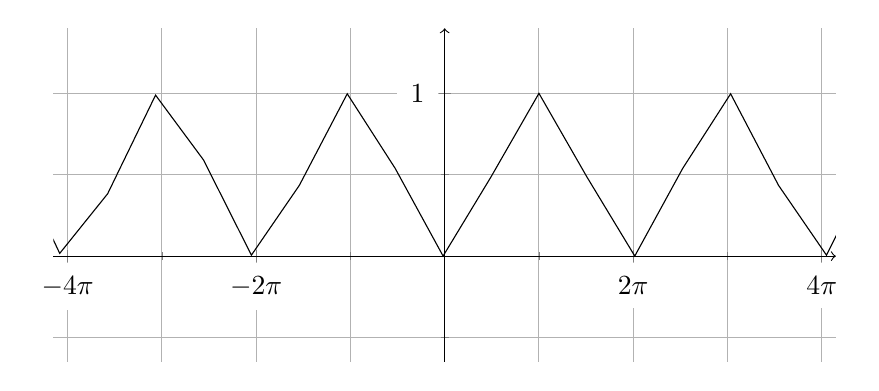
\begin{tikzpicture}[
        declare function={
          A=-0.5; B=1; C=0; D=0.5;
          f(\x)=A*cos(deg((B*\x-C)*pi))+D;
          },
        ]
        \begin{axis}[
          grid=both, %major,minor
          grid style={line width=0.375pt, draw=gray!60},
          axis lines=center,
          axis line style={->},
          xmin=-4, xmax=4,
          ymin=-0.5, ymax=1.25,
          xtick={-4,-2,...,4},
          ytick={-1,0,1},
          xticklabels={$-4\pi$, $-2\pi$,  , $2\pi$, $4\pi$},
          minor x tick num=1, xlabel=,
          minor y tick num=1, ylabel=,
          enlargelimits={abs=0.15},
          height=0.8*\axisdefaultheight, width=0.95\linewidth,
          ticklabel style={font=\normalsize,inner sep=5pt,fill=white,opacity=1.0, text opacity=1},
          every axis plot/.append style={domain=-5.1:7.1},
          ]
          \addplot[<->] {f(x)};
        \end{axis}
      \end{tikzpicture}
    \end{center}
    \vspace*{\stretch{1}}
  \end{ex*}

  \begin{ex*}
    Determine an equation for the following sinusoidal function:

    \begin{center}
      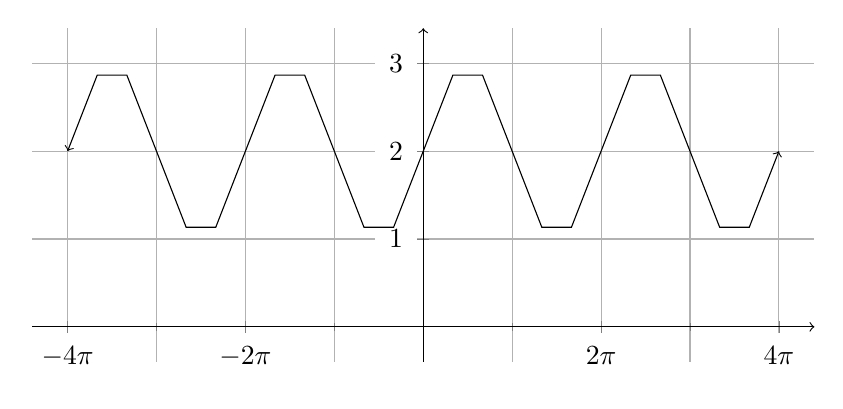
\begin{tikzpicture}[
        declare function={
          A=1; B=1; C=0; D=2;
          f(\x)=A*sin(deg((B*\x-C)*pi))+D;
          },
        ]
        \begin{axis}[
          grid=both, %major,minor
          grid style={line width=0.375pt, draw=gray!60},
          axis lines=center,
          axis line style={->},
          xmin=-4.25, xmax=4.25,
          ymin=-0.25, ymax=3.25,
          xtick={-4,-2,...,4},
          xticklabels={$-4\pi$, $-2\pi$, , $2\pi$, $4\pi$},
          minor x tick num=1, xlabel=,
          ylabel=,
          enlargelimits={abs=0.15},
          height=0.8*\axisdefaultheight, width=0.95\linewidth,
          ticklabel style={font=\normalsize,inner sep=5pt,fill=white,opacity=1.0, text opacity=1},
          every axis plot/.append style={domain=-4:4},
          ]
          \addplot[<->] {f(x)};
        \end{axis}
      \end{tikzpicture}
    \end{center}
    \vspace*{\stretch{1}}
  \end{ex*}
  \pagebreak

  \begin{ex*}
    Determine an equation for the following sinusoidal function:

    \begin{center}
      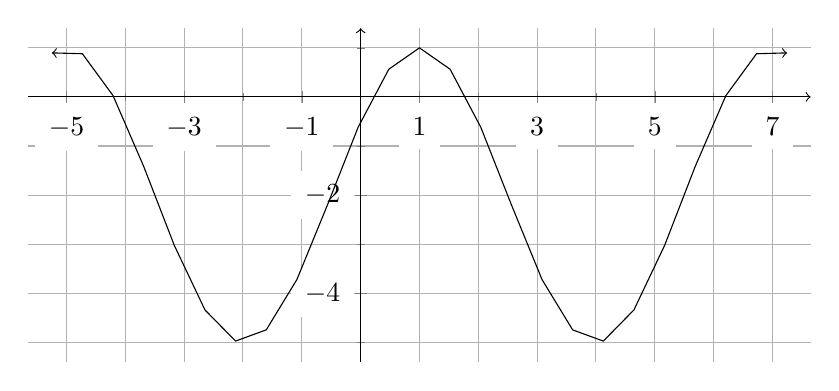
\begin{tikzpicture}[
        declare function={
          A=3; B=pi/3; C=pi/3; D=-2;
          f(\x)=A*cos(deg((B*\x-C)))+D;
          },
        ]
        \begin{axis}[
          grid=both, %major,minor
          grid style={line width=0.375pt, draw=gray!60},
          axis lines=center,
          axis line style={->},
          xmin=-5.5, xmax=7.5,
          ymin=-5.25, ymax=1.25,
          xtick={-5,-3,...,7},
          minor x tick num=1, 
          xlabel=,
          minor y tick num=1, ylabel=,
          enlargelimits={abs=0.15},
          height=0.8*\axisdefaultheight, width=0.95\linewidth,
          ticklabel style={font=\normalsize,inner sep=5pt,fill=white,opacity=1.0, text opacity=1},
          every axis plot/.append style={domain=-5.25:7.25},
          ]
          \addplot[<->] {f(x)};
        \end{axis}
      \end{tikzpicture}
    \end{center}
    \vspace*{\stretch{1}}
  \end{ex*}

  \begin{ex*}
    Determine an equation for the following sinusoidal function:

    \begin{center}
      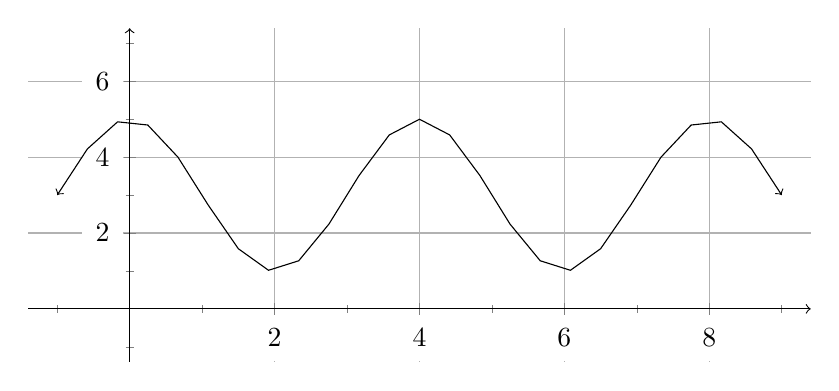
\begin{tikzpicture}[
        declare function={
          A=-2; B=1/2; C=-1; D=3;
          f(\x)=A*cos(deg((B*\x-C)*pi))+D;
          },
        ]
        \begin{axis}[
          grid=major, %major,minor,both
          grid style={line width=0.375pt, draw=gray!60},
          axis lines=center,
          axis line style={->},
          xmin=-1.25, xmax=9.25,
          ymin=-1.25, ymax=7.25,
          xtick={-2,0,...,10},
          minor x tick num=1, xlabel=,
          minor y tick num=1, ylabel=,
          enlargelimits={abs=0.15},
          height=0.8*\axisdefaultheight, width=0.95\linewidth,
          ticklabel style={font=\normalsize,inner sep=5pt,fill=white,opacity=1.0, text opacity=1},
          every axis plot/.append style={domain=-1:9},
          ]
          \addplot[<->] {f(x)};
        \end{axis}
      \end{tikzpicture}
    \end{center}
    \vspace*{\stretch{1}}
  \end{ex*}

  \pagebreak
\end{document}
